\documentclass[tikz,border=2pt]{standalone}
\usepackage{pgfplots}
\pgfplotsset{compat=1.7}

\begin{document}
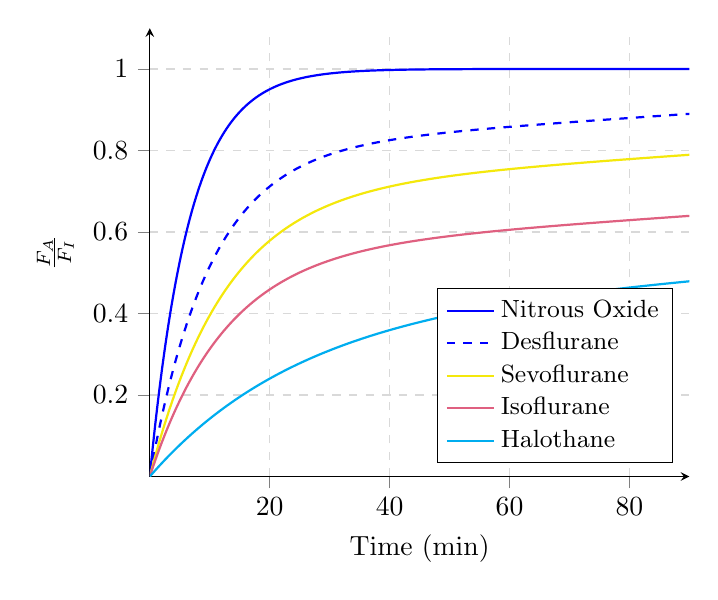
\begin{tikzpicture}


\begin{axis}[
        axis lines=middle,
	ymin = 0,
	ymax = 1.1,
	xmin = 0,
xmax = 90,
        grid = major,
        grid style={dashed, gray!30},
	 ylabel near ticks,
	xlabel near ticks,
        xlabel=Time (min),
        ylabel=$\frac{F_A}{F_I}$,
        tick align=outside,
        enlargelimits=false,
legend pos= south east,
legend style={font=\small, cells={align=left}},
legend cell align={left}]

\plot[domain=0:90, blue, thick,samples=500] {1-exp(-0.15*x)};
\addlegendentry{Nitrous Oxide}
\plot[domain=0:90, blue, dashed, thick,samples=500] {0.8*(1-exp(-0.1*x)) +0.001*x};
\addlegendentry{Desflurane}
\plot[domain=0:90, yellow!95!black, thick,samples=500] {0.7*(1-exp(-0.08*x)) +0.001*x};
\addlegendentry{Sevoflurane}
\plot[domain=0:90, pink!50!purple, thick,samples=500] {0.55*(1-exp(-0.08*x)) +0.001*x};
\addlegendentry{Isoflurane}
\plot[domain=0:90, cyan, thick,samples=500] {0.4*(1-exp(-0.04*x)) +0.001*x};
\addlegendentry{Halothane}
\end{axis}

\end{tikzpicture} 
\end{document}